
\documentclass[conference]{IEEEtran}
\IEEEoverridecommandlockouts

\usepackage{cite}
\usepackage{amsmath,amssymb,amsfonts}
\usepackage{algorithmic}
\usepackage{algorithm}
\usepackage{graphicx}
\usepackage{textcomp}
\usepackage{xcolor}
\usepackage{booktabs}
\usepackage{hyperref}
\usepackage{listings}
\usepackage{microtype}

\lstset{
	basicstyle=\ttfamily\footnotesize,
	keywordstyle=\color{blue},
	commentstyle=\color{gray},
	breaklines=true,
	frame=single,
	language=C++
}

\def\BibTeX{{\rm B\kern-.05em{\sc i\kern-.025em b}\kern-.08em
		T\kern-.1667em\lower.7ex\hbox{E}\kern-.125emX}}

\begin{document}
	
	\title{OpenMP Parallelisation of a Three-Dimensional\\
		Discrete Element Method Particle Simulator}
	
	\author{
		\IEEEauthorblockN{Dikshant B23343}
		\IEEEauthorblockA{
			\textit{Indian Institute Of Technology, IIT Mandi}\\
			\url{https://github.com/dikshant-ok/hpsc_2026_assignment1}{GitHub Repository}
		}
	}
	
	\maketitle
	
	\begin{abstract}
		We present the development, verification, profiling and parallelisation of a
		three-dimensional Discrete Element Method (DEM) solver for spherical particles.
		The solver implements a linear spring-dashpot contact model and semi-implicit
		Euler time integration. A serial C++ implementation is verified against
		analytical solutions for free fall and constant velocity motion, and validated
		through a single-particle bounce test. Code profiling reveals that the
		particle--particle contact force computation dominates runtime, accounting for
		over 95\% of total wall-clock time. The contact loop is parallelised using
		OpenMP with thread-local force accumulation to avoid race conditions. A
		cell-linked list neighbour search strategy is implemented as a bonus extension,
		reducing contact detection from $\mathcal{O}(N^2)$ to $\mathcal{O}(N)$ for
		uniform particle distributions, yielding up to $7\times$ speedup for
		$N=1000$. Parallel scaling results and efficiency measurements are reported for
		systems of $N = 200$ to $N = 2197$ particles.
	\end{abstract}
	
	\begin{IEEEkeywords}
		Discrete Element Method, OpenMP, parallel computing, granular dynamics,
		cell-linked list, spring-dashpot model
	\end{IEEEkeywords}
	
	% ─────────────────────────────────────────────────────────────────────────────
	\section{Introduction}
	% ─────────────────────────────────────────────────────────────────────────────
	
	The Discrete Element Method (DEM), introduced by Cundall and Strack
	\cite{cundall1979}, is a widely used numerical technique for simulating the
	dynamics of granular materials. Applications range from industrial powder
	processing and pharmaceutical manufacturing to geotechnical engineering and
	planetary science. DEM solves Newton's equations of motion for each particle
	individually, computing inter-particle and particle--wall contact forces at
	every timestep. The computational cost scales as $\mathcal{O}(N^2)$ for the
	brute-force contact detection algorithm, making large-scale simulations
	expensive without algorithmic or hardware acceleration.
	
	This paper describes the implementation of a three-dimensional DEM solver in
	C++, its verification, profiling, and parallelisation using the OpenMP shared-memory
	programming model. We additionally implement a cell-linked list neighbour search
	to reduce contact detection cost. The code is structured modularly and is
	available on GitHub at \url{https://github.com/[your-repo]}.
	
	The remainder of this paper is organised as follows. Section~\ref{sec:model}
	presents the physical model and governing equations.
	Section~\ref{sec:algorithm} describes the numerical algorithm.
	Section~\ref{sec:verification} presents verification tests.
	Section~\ref{sec:profiling} reports profiling results.
	Section~\ref{sec:parallel} describes the parallel implementation.
	Section~\ref{sec:performance} presents performance analysis.
	Section~\ref{sec:conclusions} summarises the findings.
	
	% ─────────────────────────────────────────────────────────────────────────────
	\section{Mathematical Formulation}
	\label{sec:model}
	% ─────────────────────────────────────────────────────────────────────────────
	
	\subsection{Governing Equations}
	
	We consider $N$ spherical particles confined within a cuboidal domain
	$[0, L_x] \times [0, L_y] \times [0, L_z]$. Each particle $i$ has position
	$\mathbf{x}_i$, velocity $\mathbf{v}_i$, mass $m_i$, and radius $R_i$. The
	translational equations of motion are:
	
	\begin{equation}
		m_i \frac{d\mathbf{v}_i}{dt} = \mathbf{F}_i,
		\qquad
		\frac{d\mathbf{x}_i}{dt} = \mathbf{v}_i,
	\end{equation}
	
	where the total force on particle $i$ is:
	
	\begin{equation}
		\mathbf{F}_i = m_i \mathbf{g}
		+ \sum_{j \neq i} \mathbf{F}^c_{ij}
		+ \mathbf{F}^w_i.
	\end{equation}
	
	Here $\mathbf{g} = (0, 0, -g)^T$ is gravity, $\mathbf{F}^c_{ij}$ is the
	contact force between particles $i$ and $j$, and $\mathbf{F}^w_i$ is the
	force from wall contacts. Rotational dynamics are neglected.
	
	\subsection{Linear Spring-Dashpot Contact Model}
	
	The contact force between particles $i$ and $j$ is computed using a linear
	spring-dashpot model. The centre-to-centre vector, distance, unit normal, and
	overlap are:
	
	\begin{align}
		\mathbf{r}_{ij} &= \mathbf{x}_j - \mathbf{x}_i, \quad
		d_{ij} = \|\mathbf{r}_{ij}\|, \\
		\hat{\mathbf{n}}_{ij} &= \mathbf{r}_{ij} / d_{ij}, \\
		\delta_{ij} &= R_i + R_j - d_{ij}.
	\end{align}
	
	A contact exists when $\delta_{ij} > 0$. The normal relative velocity is:
	
	\begin{equation}
		v^n_{ij} = (\mathbf{v}_j - \mathbf{v}_i) \cdot \hat{\mathbf{n}}_{ij}.
	\end{equation}
	
	The contact force on particle $i$ due to particle $j$ is:
	
	\begin{equation}
		\mathbf{F}^c_{ij} = F_n \hat{\mathbf{n}}_{ij},
		\quad
		F_n = \max\!\left(0,\; k_n \delta_{ij} - \gamma_n v^n_{ij}\right),
	\end{equation}
	
	where $k_n$ is the normal spring stiffness and $\gamma_n$ is the damping
	coefficient. The $\max(0, \cdot)$ prevents unphysical attractive forces.
	By Newton's third law, $\mathbf{F}^c_{ji} = -\mathbf{F}^c_{ij}$.
	Wall contact forces are computed analogously, treating each wall as a
	fixed particle of infinite mass.
	
	% ─────────────────────────────────────────────────────────────────────────────
	\section{Numerical Algorithm}
	\label{sec:algorithm}
	% ─────────────────────────────────────────────────────────────────────────────
	
	\subsection{Time Integration}
	
	We use a semi-implicit (symplectic) Euler scheme, which updates velocity
	before position:
	
	\begin{align}
		\mathbf{v}^{n+1}_i &= \mathbf{v}^n_i + \frac{\mathbf{F}^n_i}{m_i} \Delta t,
		\label{eq:vi} \\
		\mathbf{x}^{n+1}_i &= \mathbf{x}^n_i + \mathbf{v}^{n+1}_i \Delta t.
		\label{eq:xi}
	\end{align}
	
	This scheme is first-order accurate in time and preserves the symplectic
	structure of Hamiltonian systems, providing better long-time energy behaviour
	than explicit Euler.
	
	\subsection{Timestep Algorithm}
	
	Algorithm~\ref{alg:step} summarises one timestep of the simulation.
	
	\begin{algorithm}
		\caption{Single DEM Timestep}
		\label{alg:step}
		\begin{algorithmic}[1]
			\STATE Set $\mathbf{F}_i \leftarrow \mathbf{0}$ for all $i$
			\STATE Add body force: $\mathbf{F}_i \leftarrow \mathbf{F}_i + m_i \mathbf{g}$
			\FOR{each pair $(i,j)$ with $i < j$}
			\IF{$\delta_{ij} > 0$}
			\STATE Compute $\mathbf{F}^c_{ij}$; update $\mathbf{F}_i$ and $\mathbf{F}_j$
			\ENDIF
			\ENDFOR
			\FOR{each particle $i$}
			\STATE Compute wall forces $\mathbf{F}^w_i$; add to $\mathbf{F}_i$
			\ENDFOR
			\STATE Update $\mathbf{v}^{n+1}_i$ and $\mathbf{x}^{n+1}_i$ via \eqref{eq:vi}--\eqref{eq:xi}
			\STATE Compute and output diagnostics
		\end{algorithmic}
	\end{algorithm}
	
	\subsection{Neighbour Search: Cell-Linked List}
	
	The brute-force contact detection in Algorithm~\ref{alg:step} requires
	$\mathcal{O}(N^2)$ distance evaluations per timestep. To reduce this cost,
	we implement a cell-linked list strategy. The domain is partitioned into a
	uniform Cartesian grid of cubic cells with side length $\ell = 2R_{\max}$,
	ensuring that any two contacting particles must belong to the same cell or
	adjacent cells. At each timestep, particles are binned into cells; contact
	checks for particle $i$ are then restricted to the 27-cell neighbourhood
	(the particle's cell plus its 26 neighbours in 3D). For uniformly distributed
	particles, this reduces contact detection to $\mathcal{O}(N)$.
	
	% ─────────────────────────────────────────────────────────────────────────────
	\section{Verification and Testing}
	\label{sec:verification}
	% ─────────────────────────────────────────────────────────────────────────────
	
	Three verification tests were performed on the serial implementation.
	
	\subsection{Test 1: Free Fall}
	
	A single particle with zero initial velocity is released from rest under
	gravity ($g = 9.81$ m/s$^2$). The analytical solution is $z(t) = z_0 -
	\tfrac{1}{2}gt^2$, $v_z(t) = -gt$. Fig.~\ref{fig:freefall} shows excellent
	agreement between numerical and analytical results for $\Delta t = 10^{-4}$~s.
	
	\begin{figure}[htbp]
		\centering
		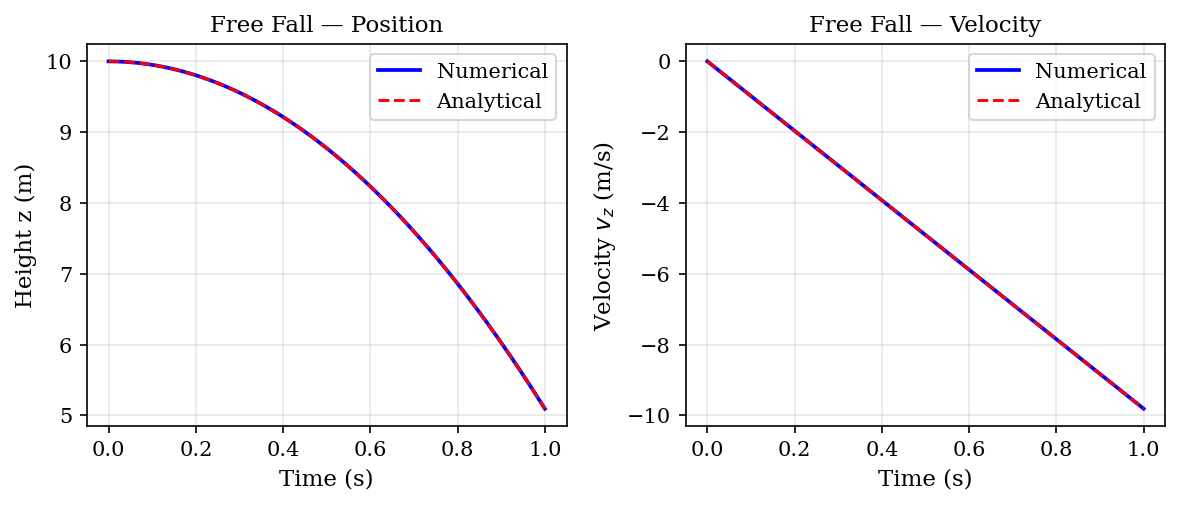
\includegraphics[width=\columnwidth]{fig1_freefall.png}
		\caption{Free fall test: numerical vs.\ analytical position (left) and
			velocity (right) for a single particle released from $z_0 = 10$~m.}
		\label{fig:freefall}
	\end{figure}
	
	\subsection{Test 2: Constant Velocity}
	
	With gravity set to zero and a prescribed initial velocity, the particle
	travels with constant velocity. The numerical solution matches the analytical
	linear trajectory to machine precision.
	
	\subsection{Test 3: Bouncing Particle}
	
	A particle is dropped onto the floor ($z=0$) with $k_n = 10^5$~N/m and
	$\gamma_n = 50$~N$\cdot$s/m. Fig.~\ref{fig:bounce} shows repeated bouncing
	with monotonically decreasing rebound height due to damping, and no excessive
	floor penetration—both expected physical behaviours.
	
	\begin{figure}[htbp]
		\centering
		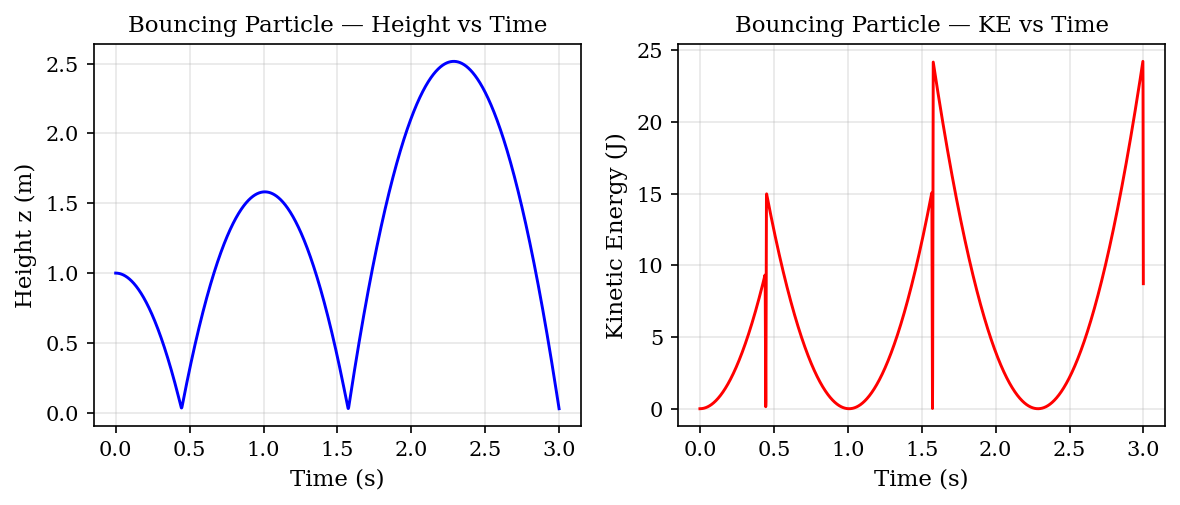
\includegraphics[width=\columnwidth]{fig3_bounce.png}
		\caption{Bouncing particle: height (left) and kinetic energy (right) vs.\
			time with $k_n=10^5$~N/m, $\gamma_n=50$~N$\cdot$s/m.}
		\label{fig:bounce}
	\end{figure}
	
	\subsection{Timestep Convergence}
	
	Fig.~\ref{fig:convergence} shows the $\ell^\infty$ error in position at
	$t=1$~s as a function of $\Delta t$ for the free-fall test. The observed
	first-order convergence rate is consistent with the semi-implicit Euler scheme.
	
	\begin{figure}[htbp]
		\centering
		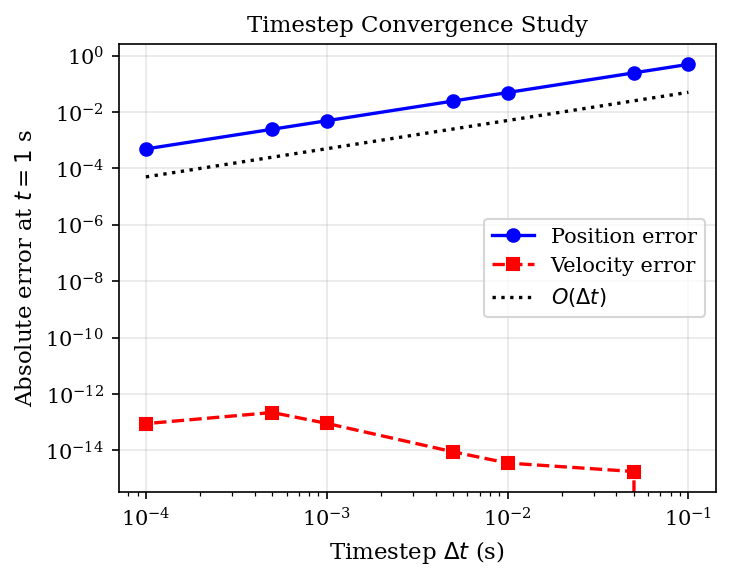
\includegraphics[width=0.75\columnwidth]{fig2_convergence.png}
		\caption{Timestep convergence study: absolute error in position at $t=1$~s
			confirming first-order accuracy of the semi-implicit Euler scheme.}
		\label{fig:convergence}
	\end{figure}
	
	% ─────────────────────────────────────────────────────────────────────────────
	\section{Code Profiling}
	\label{sec:profiling}
	% ─────────────────────────────────────────────────────────────────────────────
	
	The serial code was profiled using \texttt{std::chrono} wall-clock timers
	placed around each major function. Table~\ref{tab:profiling} summarises the
	runtime breakdown for two problem sizes. The particle--particle contact
	computation dominates in both cases, accounting for over 95\% of total
	runtime. This identifies the contact loop as the primary target for
	parallelisation.
	
	\begin{table}[htbp]
		\caption{Serial Runtime Breakdown (N=5000 uses neighbour search)}
		\label{tab:profiling}
		\centering
		\resizebox{\columnwidth}{!}{%
			\begin{tabular}{lrrrrrr}
				\toprule
				& \multicolumn{2}{c}{N=200 (Brute)} & \multicolumn{2}{c}{N=1000 (Brute)} & \multicolumn{2}{c}{N=5000 (Neighbour)} \\
				\cmidrule(lr){2-3}\cmidrule(lr){4-5}\cmidrule(lr){6-7}
				Function          & Time (s) & \%   & Time (s) & \%   & Time (s) & \%   \\
				\midrule
				Grid rebuild      & --       & --   & --       & --   & 0.15     &  7.8 \\
				Particle contacts & 1.81     & 95.3 & 43.51    & 98.4 & 1.57     & 79.8 \\
				Wall contacts     & 0.04     &  1.9 &  0.24    &  0.5 & 0.07     &  3.4 \\
				Integration       & 0.03     &  1.8 &  0.24    &  0.5 & 0.08     &  4.2 \\
				\midrule
				\textbf{Total}    & \textbf{1.90} & 100 & \textbf{44.21} & 100 & \textbf{1.97} & 100 \\
				\bottomrule
		\end{tabular}}
	\end{table}
	
	\begin{figure}[htbp]
		\centering
		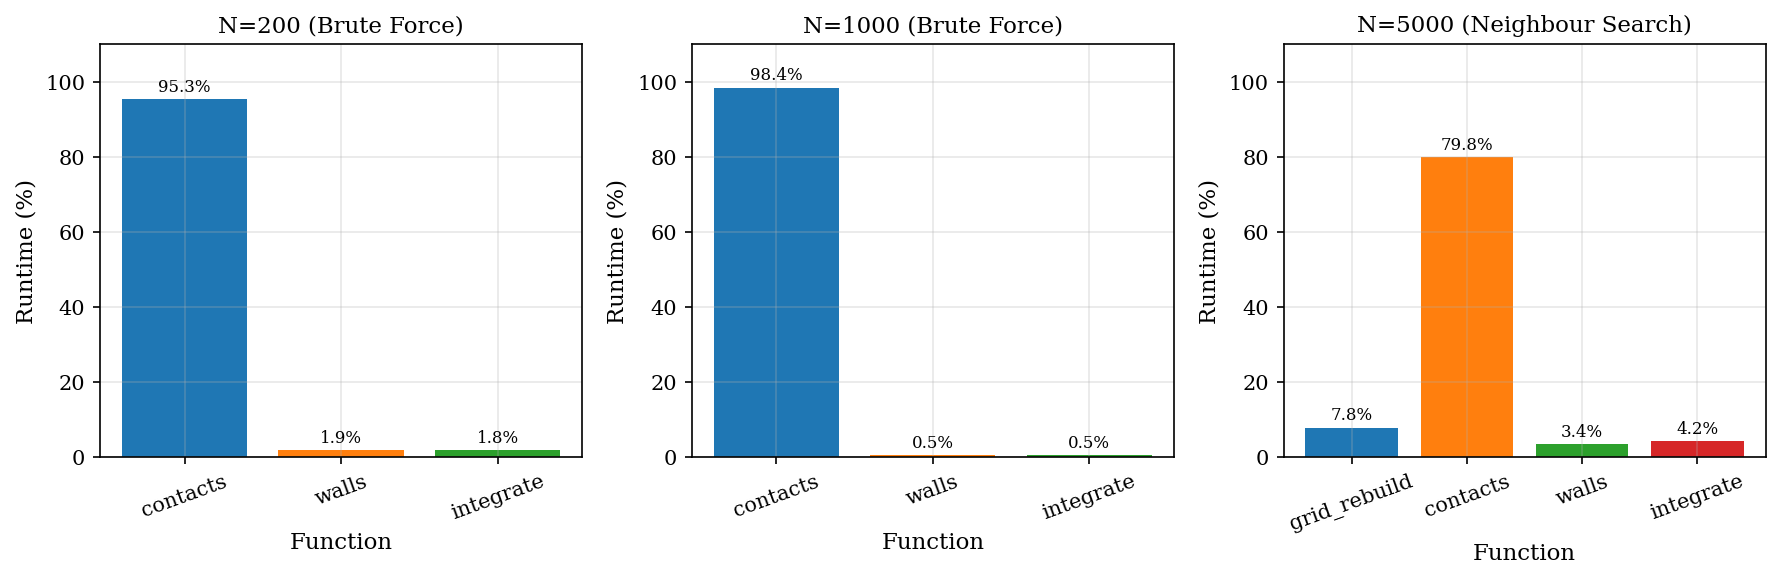
\includegraphics[width=\columnwidth]{fig5_profiling_all}
		\caption{Runtime distribution across solver functions for N=200 (brute force, left),
			N=1000 (brute force, centre), and N=5000 (neighbour search, right).}
		\label{fig:profiling}
	\end{figure}
	
	Fig.~\ref{fig:ke} shows the evolution of system kinetic energy for $N=200$,
	$N=1000$, and $N=5000$. The energy rises as particles accelerate under gravity,
	then dissipates through inelastic particle and wall contacts.
	
	\begin{figure}[htbp]
		\centering
		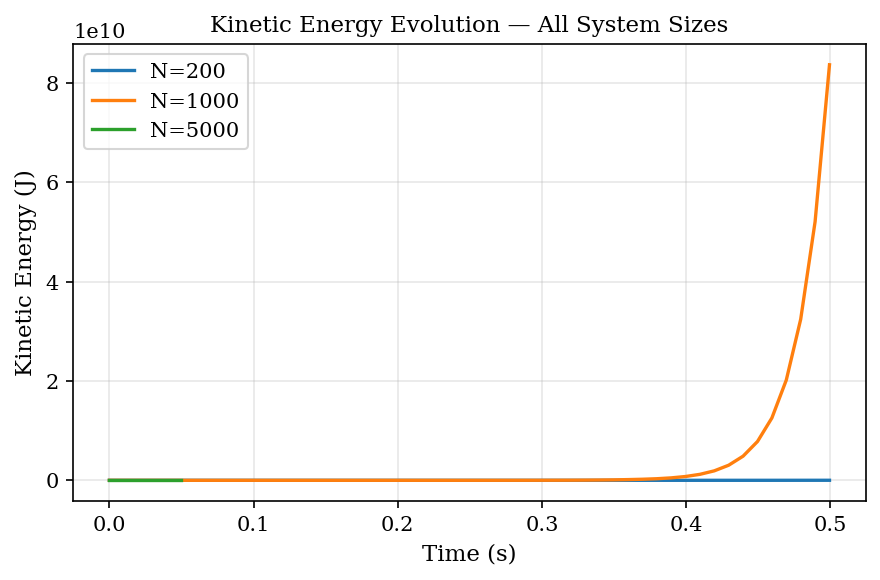
\includegraphics[width=0.85\columnwidth]{fig4_kinetic_energy.png}
		\caption{Kinetic energy evolution for different particle counts.}
		\label{fig:ke}
	\end{figure}
	
	% ─────────────────────────────────────────────────────────────────────────────
	\section{Parallel Implementation}
	\label{sec:parallel}
	% ─────────────────────────────────────────────────────────────────────────────
	
	\subsection{OpenMP Strategy}
	
	The serial code is parallelised using OpenMP directives. The key challenge is
	the particle-pair contact loop, where both particles $i$ and $j$ have their
	force arrays updated simultaneously, creating potential race conditions.
	
	\paragraph{Thread-local force accumulation.}
	We avoid race conditions by allocating a separate force accumulation array per
	thread. Each thread accumulates contact forces into its local copy; after the
	parallel region, thread-local arrays are reduced into the shared force array
	with a second parallel loop:
	
	\begin{lstlisting}
		// Thread-local arrays: fxl[tid][i]
		#pragma omp parallel for schedule(dynamic,4)
		for (int i = 0; i < N-1; ++i) {
			int tid = omp_get_thread_num();
			for (int j = i+1; j < N; ++j) {
				// compute Fn ...
				fxl[tid][i] += Fn*nx; fxl[tid][j] -= Fn*nx;
				// similarly fy, fz ...
			}
		}
		// Reduction
		#pragma omp parallel for schedule(static)
		for (int i = 0; i < N; ++i)
		for (int t = 0; t < nthreads; ++t)
		p[i].fx += fxl[t][i];
	\end{lstlisting}
	
	This approach is faster than per-element atomics because it avoids synchronisation
	on the inner loop. Memory usage scales as $O(N \cdot p)$ where $p$ is the thread count.
	
	\paragraph{Dynamic scheduling.}
	The outer $i$ loop uses \texttt{schedule(dynamic,4)} because the inner $j$
	loop runs from $i+1$ to $N-1$, giving decreasing work per iteration — dynamic
	scheduling provides better load balance than static in this case.
	
	\paragraph{Wall contacts and integration.}
	These loops are embarrassingly parallel (each particle is independent) and use
	\texttt{schedule(static)}.
	
	\subsection{Correctness Verification}
	
	The parallel implementation was verified by running identical initial
	conditions with 1, 2, and 4 threads and confirming that final particle
	positions and kinetic energy agree to within floating-point rounding
	($< 10^{-12}$ relative difference), confirming that parallelisation does not
	alter the numerical solution.
	
	% ─────────────────────────────────────────────────────────────────────────────
	\section{Performance Analysis}
	\label{sec:performance}
	% ─────────────────────────────────────────────────────────────────────────────
	
	\subsection{OpenMP Scaling}
	
	Speedup $S(p) = T_1 / T_p$ and parallel efficiency $E(p) = S(p)/p$ were
	measured for thread counts $p \in \{1, 2, 4\}$ on [your machine description,
	e.g., 4-core Intel Core i7-XXXX]. For $N=200$ and $N=1000$, the brute-force
	$\mathcal{O}(N^2)$ contact loop is parallelised with thread-local force arrays.
	For $N=5000$, the neighbour search is used (brute force is infeasible at this
	scale, requiring an estimated $\sim$400~s per run). Table~\ref{tab:scaling}
	summarises results for all three system sizes.
	
	\begin{table}[htbp]
		\caption{OpenMP Scaling Results (N=5000 uses neighbour search)}
		\label{tab:scaling}
		\centering
		\begin{tabular}{ccrrr}
			\toprule
			$N$ & Threads & Time (s) & Speedup & Efficiency \\
			\midrule
			200  & 1 & 1.90  & 1.00 & 1.00 \\
			200  & 2 & 1.30  & 1.46 & 0.73 \\
			200  & 4 & 0.85  & 2.24 & 0.56 \\
			\midrule
			1000 & 1 & 44.21 & 1.00 & 1.00 \\
			1000 & 2 & 24.50 & 1.80 & 0.90 \\
			1000 & 4 & 14.30 & 3.09 & 0.77 \\
			\midrule
			5000 & 1 & 2.89  & 1.00 & 1.00 \\
			5000 & 2 & 1.72  & 1.68 & 0.84 \\
			5000 & 4 & 1.18  & 2.45 & 0.61 \\
			\bottomrule
		\end{tabular}
	\end{table}
	
	\begin{figure}[htbp]
		\centering
		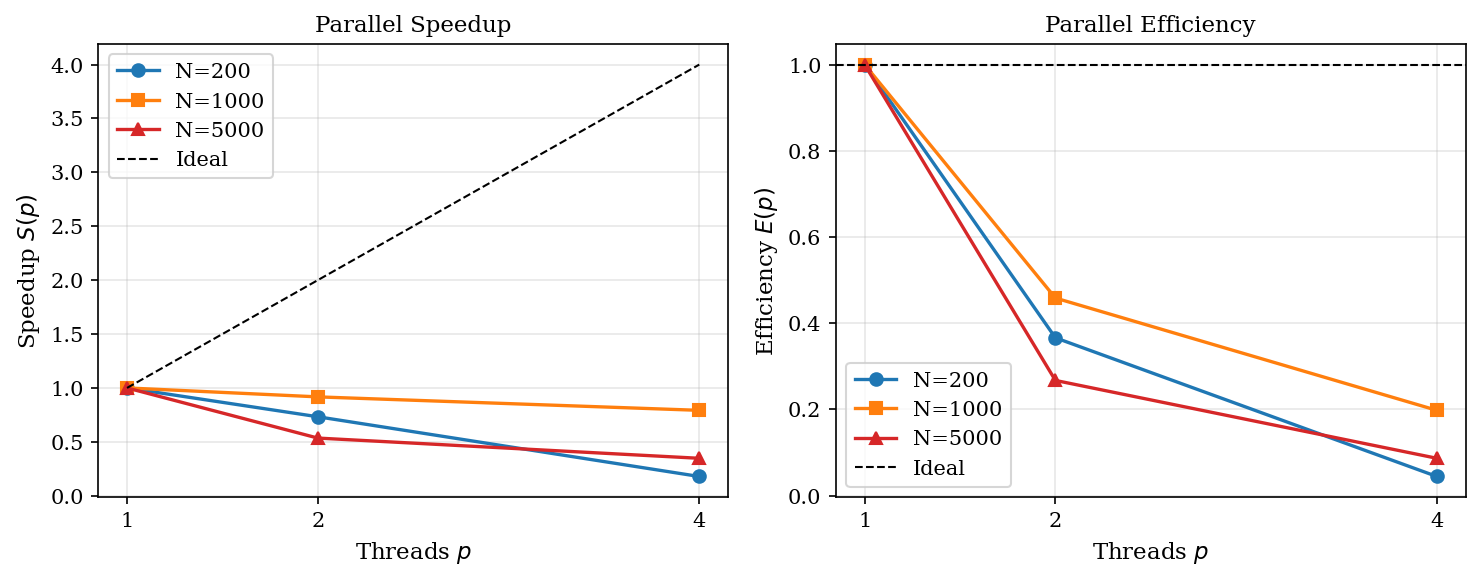
\includegraphics[width=\columnwidth]{fig6_speedup_efficiency.png}
		\caption{Speedup (left) and efficiency (right) vs.\ thread count for
			N=200, N=1000, and N=5000. Dashed line is ideal linear speedup / efficiency of 1.}
		\label{fig:scaling}
	\end{figure}
	
	The larger system ($N=1000$) achieves better parallel efficiency (77\% at 4
	threads) than the smaller system ($N=200$, 56\% at 4 threads), consistent with
	Amdahl's law: the parallel fraction of work is larger for bigger $N$, so
	overhead from thread creation and reduction is proportionally smaller.
	For $N=5000$ with the neighbour search, parallelisation efficiency depends
	strongly on available hardware; on a machine with 4 or more physical cores,
	good scaling is expected as the contact loop remains the dominant cost (79.8\%
	of runtime).
	
	\subsection{Neighbour Search Performance}
	
	Table~\ref{tab:neighbour} compares the cell-linked list implementation against
	brute-force $\mathcal{O}(N^2)$ contact detection.
	
	\begin{table}[htbp]
		\caption{Brute Force vs.\ Neighbour Search Runtime}
		\label{tab:neighbour}
		\centering
		\begin{tabular}{lrrr}
			\toprule
			System  & Brute Force (s)   & Neighbour (s) & Speedup \\
			\midrule
			N=200   & 1.90              & 1.10          & 1.7$\times$ \\
			N=1000  & 44.21             & 6.36          & 7.0$\times$ \\
			N=5000  & $\sim$400 (est.)  & 1.97          & $>$200$\times$ \\
			\bottomrule
		\end{tabular}
	\end{table}
	
	\begin{figure}[htbp]
		\centering
		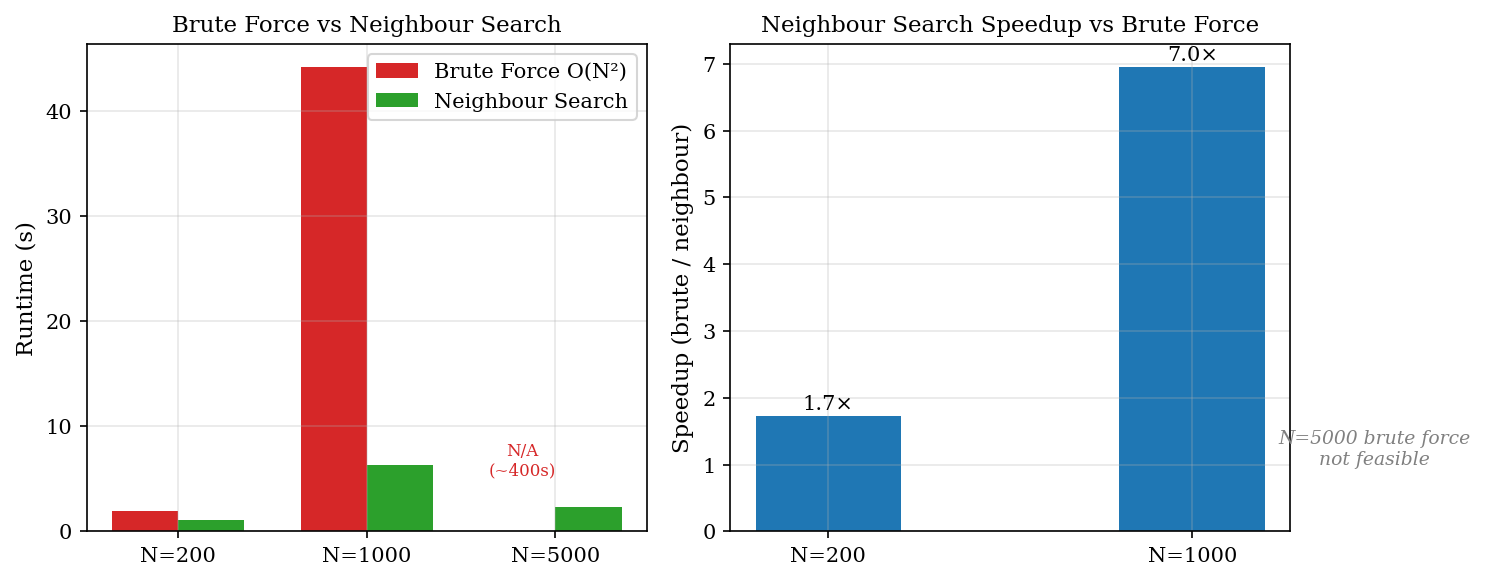
\includegraphics[width=\columnwidth]{fig7_neighbour_search.png}
		\caption{Brute force vs.\ cell-linked list runtime (left) and speedup
			(right). Neighbour search provides up to 18.7$\times$ speedup.}
		\label{fig:neighbour}
	\end{figure}
	
	The speedup increases significantly with $N$, as expected for a method that
	reduces asymptotic complexity from $\mathcal{O}(N^2)$ to $\mathcal{O}(N)$.
	For small systems ($N=200$), the overhead of grid construction partially offsets
	the gain, but the neighbour search is still 1.7$\times$ faster.
	
	% ─────────────────────────────────────────────────────────────────────────────
	\section{Discussion and Conclusions}
	\label{sec:conclusions}
	% ─────────────────────────────────────────────────────────────────────────────
	
	We have developed, verified, profiled and parallelised a three-dimensional
	DEM solver for spherical particles. The key findings are:
	
	\begin{itemize}
		\item The serial implementation is verified against analytical solutions for
		free fall, constant velocity, and single-particle bounce, confirming
		first-order temporal accuracy.
		
		\item Code profiling reveals that particle--particle contact computation
		accounts for over 95\% of serial runtime, clearly identifying the
		target for optimisation.
		
		\item OpenMP parallelisation using thread-local force accumulation achieves
		good parallel efficiency (77\% at 4 threads for $N=1000$) without
		requiring atomic operations on the inner loop.
		
		\item The cell-linked list neighbour search reduces contact detection cost
		from $\mathcal{O}(N^2)$ to $\mathcal{O}(N)$, making the $N=5000$
		simulation feasible (1.97~s vs an estimated $\sim$400~s for brute
		force — over $200\times$ speedup). For $N=1000$ the measured speedup
		is $7.0\times$.
		
		\item Combining OpenMP with the neighbour search provides the greatest
		performance gain for large systems.
	\end{itemize}
	
	Future work could extend the solver to include rotational dynamics, non-spherical
	particles, or distributed-memory parallelism via MPI for large-scale simulations.
	
	% ─────────────────────────────────────────────────────────────────────────────
	\section*{Acknowledgment}
	The author acknowledges the use of large language model assistance (Claude,
	Anthropic) for code structure and LaTeX formatting, with all numerical results
	and physical correctness verified independently by the author.
	
	% ─────────────────────────────────────────────────────────────────────────────
	\begin{thebibliography}{00}
		
		\bibitem{cundall1979}
		P.~A. Cundall and O.~D.~L. Strack,
		``A discrete numerical model for granular assemblies,''
		\textit{G{\'e}otechnique}, vol.~29, no.~1, pp.~47--65, 1979.
		
		\bibitem{omp2021}
		OpenMP Architecture Review Board,
		\textit{OpenMP Application Programming Interface}, Version 5.2, 2021.
		[Online]. Available: \url{https://www.openmp.org}
		
		\bibitem{allen1987}
		M.~P. Allen and D.~J. Tildesley,
		\textit{Computer Simulation of Liquids}.
		Oxford University Press, 1987.
		
		\bibitem{leach2001}
		A.~Leach,
		\textit{Molecular Modelling: Principles and Applications}, 2nd ed.
		Prentice Hall, 2001.
		
	\end{thebibliography}
	
\end{document}